%!TEX root = ../template.tex
%%%%%%%%%%%%%%%%%%%%%%%%%%%%%%%%%%%%%%%%%%%%%%%%%%%%%%%%%%%%%%%%%%%
%% chapter1.tex
%% NOVA thesis document file
%%
%% Chapter with introduction
%%%%%%%%%%%%%%%%%%%%%%%%%%%%%%%%%%%%%%%%%%%%%%%%%%%%%%%%%%%%%%%%%%%
\newcommand{\novathesis}{\emph{novathesis}}
\newcommand{\novathesisclass}{\texttt{novathesis.cls}}


\chapter{Introduction}
\label{cha:introduction}

\begin{quotation}
\begin{flushright}
\itshape
«“Begin at the beginning," the King said, very gravely, \\"and go on till you come to the end: then stop.”»\\
\textbf{- Lewis Carroll, Alice in Wonderland}
\end{flushright}
\end{quotation}

Health is one of the pillars of well-being. Although very precious, health is volatile and subject to constant disturbances imposed by disease and injury. One such type of disturbance is caused by burn injuries. Burn injury still has an expression worldwide as a cause of death and contribute heavily to morbidity and disability.

The healthcare system is responsible to apply scientific methods and tools to reduce the impacts of disease and injury and re-establish health. The development of new methods and tools that help attaining that goal is always desirable. As other scientific fields develop, new possibilities emerge from the combination of different knowledge. This symbiosis inspires the creation of new tools and the introduction of new procedures to improve healthcare.

This work presents a tool concept which results from the combination of different scientific fields, with the goal of improving the treatment of various types of skin wounds, in particular the case of burn injuries.\\

Next, on this chapter, a brief overview of the reality of burn injury will be presented. Afterwards, a case is made to show that the development of three independent scientific fields allows the development of the tool concept presented by this thesis. The goal of the thesis will be presented, followed by an overview of the proposed system architecture, and culminating on the summary of the document structure.

% ==============================
% = The reality of burn injury =
% ==============================
\section{The reality of burn injury} % (fold)
\label{sec:the_reality_of_burn_injury}

Burn injuries are still a prevalent problem in today's society, claiming the lives of about 17 people worldwide, every hour, by 2016 \cite{GHE2016_xls}. Although it represents a small percentage of global death numbers, burn wounds have a significant impact on morbidity and mortality and are considered the worst type of traumatic injury \cite{isbi_guidelines_burn_care}. They also represent a considerable societal cost associated with the expenses for medical care and physical or psychological rehabilitation \cite{Brusselaers_2010_europe_systematic_review}. When not leading to death, they commonly leave the person "with lifelong disabilities and disfigurements, often with resulting stigma and rejection" \cite{who2011_sucess_stories}.

Injuries result from "an uncontrolled transfer of energy to the human body in amounts that a body cannot tolerate" \cite{who2011_sucess_stories}. Burn injuries are produced by the transfer of radiation or thermal, electrical and chemical energies to the body. Some examples are direct contact with flames, hot objects or liquids (scalds); exposure to ionising radiation; or contact with high electrical currents, or chemicals \cite{who_unicef2008_burns_chapter}.

Burn wounds are typically external wounds inflicted to the skin. Only in some cases like inhalational burns and electric burns the injury is internal and affects something other than the skin.

The skin, the major part of the integumentary system, is the largest organ on the body. It covers the whole surface of the body and has several important functions. It contributes to thermal regulation; works as a protection layer (from UV radiation, microbes, mechanical and thermal offences) for the underlying tissues; acts as a sensitive layer for touch, temperature or pain; allows the excretion and absorption of water and other substances; is a blood reservoir; and synthesises vitamin D \cite{Tortora2009_principles_anatomy_physiology}. 

Concerning its structure, the skin is composed of three layers. The outermost layer is called the epidermis which is a stratified squamous epithelium. It is the main protective barrier. The middle layer is called dermis which is mostly conjunctive tissue.  It is very important because it also contains hair follicles, nerves, sebaceous and sweat glands, blood vessels, and some fat cells. Finally, the innermost layer is the hypodermis. It is mainly adipose and areolar tissues and also contains blood vessels \cite{Tortora2009_principles_anatomy_physiology}.

Various criteria are used to classify burn wounds. The mechanism or cause, the extension, and degree or depth, are the most common \cite{who_unicef2008_burns_chapter}. 

The cause of the wound is related to the energy source involved on the injury formation; It can be further classified as thermal or inhalational, to separate damaged to the skin or to the airways and lungs, respectively \cite{who_unicef2008_burns_chapter}.

The burn extension is clinically referred as the \gls{tbsa} burned, or how much surface area of the skin was burned. The most common method used to determine this quantity is called the "rule of nines". This method "assigns 9\% to the head and neck region, 9\% to each arm (including the hand), 18\% to each leg (including the foot) and 18\% to each side of the trunk (back, chest and abdomen)" \cite{who_unicef2008_burns_chapter}. It is only used for adults and children over 10 years. For younger children, the Lund and Browder Chart is used \cite{MacLennan1998_anesthesia_thermal_injury}. 

The degree or depth is a very important criteria, because it is directly related to the type of treatment applied. It is separated in three degrees: (a) first-degree, or superficial burns; (b) second-degree, or partial-thickness burns; and (c) third-degree, or full-thickness burns \cite{who_unicef2008_burns_chapter}. 

A first-degree wound only impacts the epidermis. It takes about a week to heal. Second-degree burns already affect epidermis and dermis. The healing process takes about 3 to 4 weeks but it still can heal by itself. Hair follicles, sebaceous and sweat glands are generally unaffected, but it loses some of its functions \cite{Tortora2009_principles_anatomy_physiology}. A third-degree burn wound impacts all three layers. The skin loses most of its functions \cite{Tortora2009_principles_anatomy_physiology} and it generally needs a skin graft to heal properly \cite{who_unicef2008_burns_chapter}. In some cases, a fourth-degree is referred, and it is when the injury crosses all three layers of skin and also affects the underlying tissues like fascia and muscles, or even bone \cite{Vijayavenkataraman2016_stateart_modelling_materials_processing}. 

The \gls{tbsa} and the wound depth have major impact on morbidity and mortality. Larger \gls{tbsa} and deeper wounds directly impact the need of emergency care and hospitalisation, the complexity of the treatment, and the \gls{los} \cite{Santos_2016_burden_burns_portugal, Bartosch_2013_mortality_lengthofstay}. Naturally, this increases the overall costs of treatment, and the burden of the injury. 

In Portugal, a clinical and economical analysis of burn injuries, encompassing a period of 13 years, revealed an average direct cost per year of 13 million Euros, and 6741 Euros per hospitalisation \cite{Santos_2016_burden_burns_portugal}. \gls{is}, which is one type of stroke (the second main cause of death worldwide \cite{GHE2016_xls}), has an average direct cost of hospitalisation of 2215 Euros \cite{Santos_2017_atrial_fibrillation_stroke}. Comparing the hospitalisation costs and the number of associated deaths per year, we can see that burns have a lower number deaths, but cost three times more, on average. This clearly shows the financial impact of burn wound treatment. \\ 

\begin{comment}
According to the \citeauthor{who2008_plan_burn_prevention_care} (WHO) \cite{who2011_sucess_stories}, the occurrence and outcome severity of burn injuries are higher on \gls{lmic} than on \gls{hic}, with 95\% of annual casualties happening on \gls{lmic}. The death rate in \gls{lmic} is about 6 times larger than on \gls{hic}, reaching around 5.5 deaths/100 000 people per year \cite{who2011_sucess_stories}. 

The disparity on resources between \gls{hic} and \gls{lmic} means the former has a better leverage to develop strategies to reduce the onset of burn events and lower its morbidity and mortality. Valid strategies consist of: (a) the implementation of effective prevention plans, (b) providing better first-aid and medical care, (c) the application of follow-up intervention for rehabilitation and psychological support, or (d) the development of research efforts to better understand the reality of burn injuries. \cite{who2008_plan_burn_prevention_care, who2011_sucess_stories}. The implementation of these strategies on high income countries have "effectively and sustainably" reduced the number of events and mortality over the last three to four decades \cite{who2011_sucess_stories}. 
Now, the focus of \gls{hic} is on better medical care to improve healing and reduce scarring, or to provide rehabilitation and psychological support. Restoring "form and function have become the hallmarks of excellent burn care" \cite{isbi_guidelines_burn_care}. On \gls{lmic}, the main focus should be on reducing the occurrence, morbidity and mortality. This means they need to place more effort on prevention, first-aid care and hospital care \cite{who2008_plan_burn_prevention_care, who2011_sucess_stories}.

The occurrence by cause of burn varies between \gls{hic} and \gls{lmic}. In \gls{hic} the most common cause are scalds associated with food preparation or consumption and bathing. The victims of these scalds tend to be infants younger than 5 years old. In \gls{lmic} flame burns are the most common. They are usually related with the usage of unsafe stoves and lamps. Scalds, generally, lead to non-lethal burns, however, on younger ages, in many cases it leads to death. Burns by flame are more lethal, usually having higher \gls{tbsa} and depth \cite{who2011_sucess_stories, who_unicef2008_burns_chapter}.\\
\end{comment}

The main cause of early death (within the first 24 hours) from burn injury is dehydration and shock caused by a huge loss of body fluids. If the patient survives the first day, the following main cause of death is sepsis. The fragility of the immune system, due to dysfunction of the integumentary system, renders the patients more prone to infectious diseases, such as pneumonia \cite{who2011_sucess_stories}. When a week as passed, the burn site is covered by many organisms, with the most virulent ones starting to invade the healthy tissue \cite{isbi_guidelines_burn_care}. "The avascular nature of the burn predisposes the burn site to bacterial invasion by impeding effective delivery of the antibodies’ own defences and preventing systemic antibiotics from penetrating the damaged area" \cite{isbi_guidelines_burn_care}. Several types of microbial agents have been found on burn wounds, from bacteria to virus and fungi \cite{Schaal2015a_fungal_infections,Shoja2017_acinetobacter}. If not detected and treated early, these infections can significantly impact morbidity and eventually lead to death.

To prevent microbial infections, burn wounds are first mechanically cleanse by irrigation, followed by topical application of antimicrobial cream and dressing. 

{\color{red}Need to point the importance of skin replacements to reduction infection and the time needed to heal the wound.}

Improving the quality of the burn wound care can have direct impact on treatment costs and overall outcome. The aim is to develop a treatment solution that induces rapid healing, without or with minimal scar formation, that significantly reduces the \gls{los}, morbidity and mortality. It should also be cost effective to reduce the financial impact. 

% section the_reality_of_burn_injury (end)

% ===========================================================
% = Development of complementary technologies and practices =
% ===========================================================
\section{Development of complementary technologies and practices} % (fold)
\label{sec:development_of_complementary_technologies_and_practices}

In parallel with the development of medical burn wound care, other areas of science and technology are evolving which can contribute to the improvement of treatment outcome. Three areas are emphasised on this document because they can complement each other to open new roads for treatment or intervention protocols. The areas are \textbf{three dimensional (3D) bioprinting}, \textbf{collaborative robotics}, and \textbf{computer vision}.

% = 3D Bioprinting =
\subsection{3D Bioprinting} % (fold)
\label{subsec:3D_bioprinting}

The first area, 3D bioprinting, is more directly related with the treatment itself. It is a branch of \gls{te} that as brought new perspectives on skin regeneration and healing, and holds promise of significant improvement on burn wound regeneration and scar reduction.

3D Bioprinting is an advanced manufacturing process to fabricate tissue constructs and organs via layer-by-layer deposition of cells, biomaterials and growth-factors, using \gls{cad}, in a repeatable and flexible way \cite{Ng2016_skin_bioprint_reality_fantasy}. This approach to \gls{te} was motivated by the inability of the classical approach to "fabricate complex biomimetic structures [which] results in an over-simplified tissue construct, thus rendering the engineered tissue inaccurate with unrealistic cell microenvironments" \cite{Vijayavenkataraman2018_bioprinting_tissues_organs_regen_med}. Plus, the increasing demand for organs for transplantation, the rise of bans for animal testing, and the need for better in vitro models for drug research and development, as fuelled the development of this technology \cite{Vijayavenkataraman2018_bioprinting_tissues_organs_regen_med}.

Being around for over 30 years \cite{Ozbolat2017_evaluation_bioprinter_tech}, bioprinting as attained a considerable progress in printing and testing several types of tissues. At this moment, at least a single experiment was conducted with some success pertaining any of the eleven human organ systems namely skeletal, muscular, nervous, lymphatic, endocrine, reproductive, integumentary, respiratory, digestive, urinary, and circulatory systems \cite{Vijayavenkataraman2018_bioprinting_tissues_organs_regen_med}.

This technology has some advantages like the possibility of automation; high precision on cell and material placement, geometrical freedom on the construct shape, the capability to use a wide range of materials, reproducibility, and repeatability \cite{Vijayavenkataraman2018_bioprinting_tissues_organs_regen_med}. However, like all technologies it is not without its limitations. Currently, 3D Bioprinting is not ready for full scale deployment on the healthcare sector. Although it has several reported successes, it is still on its infancy, and has a lot of room for improvement and standardisation \cite{Vijayavenkataraman2018_bioprinting_tissues_organs_regen_med, Datta2018_essential_steps_bioprinting}. To 3D bioprint a tissue construct a three stage process is followed. It starts with pre-bioprinting, followed by the bioprinting stage and ends with post-bioprinting \cite{Datta2018_essential_steps_bioprinting, Vijayavenkataraman2018_bioprinting_tissues_organs_regen_med}. 

The pre-bioprinting, or pre-processing, stage can be considered the plan phase. Imaging techniques are employed to extract precise structural information of the printing area and the organ/tissue to be printed \cite{Datta2018_essential_steps_bioprinting, Vijayavenkataraman2018_bioprinting_tissues_organs_regen_med}. Also, at this stage, the type of cells used is chosen, the cells extracted from the patient, and cell culture protocols followed to produce the cells for the bioink (some authors consider that this step is part of the bioink preparation \cite{Vijayavenkataraman2018_bioprinting_tissues_organs_regen_med}). 

On the bioprinting phase the bioinks are prepared for printing and the actual printing occurs. Different printing methods can be employed, each one with their on advantages and limitations. They are organized into three main groups: \gls{lbb}, \gls{dbb}, and \gls{ebb} \cite{Datta2018_essential_steps_bioprinting, Vijayavenkataraman2018_bioprinting_tissues_organs_regen_med}. 

The post-bioprinting, or post-processing, stage is when the tissue maturation occurs before patient transplantation or usage as an in vitro model. Several techniques can used depending on the tissue construct printed. Bioreactors are commonly used to provide a controlled environment for tissue maturation \cite{Datta2018_essential_steps_bioprinting, Vijayavenkataraman2018_bioprinting_tissues_organs_regen_med}.

All three stages have their limitations and a concerted effort of the whole community is needed to take this technology from bench to bedside. On the actual bioprinting step of the bioprinting stage some of the improvements needed are a higher number of degrees of freedom of the bioprinting system; higher printing speeds without compromising the cells viability and construct shape; and increased automation of the printing process. \cite{Ozbolat2017_evaluation_bioprinter_tech, Datta2018_essential_steps_bioprinting}. Collaborative robotics and computer vision can help solve these limitations. Next, these two fields will be introduced and some examples will be presented to show their potential to solve the aforementioned problems.

% subsection 3D_bioprinting (end)

% = Collaborative Robotics =
\subsection{Collaborative Robotics} % (fold)
\label{subsec:collaborative_robotics}

The beginning of modern robotics occurred in the early 1950s, with the invention of the first programmable manipulator, by George C. Devol. Later, together with Joseph Engelberger, Devol created the first robot manufacturing company. At 1961, their work culminated on the first industrial robot being installed at a General Motors' plant. This was the first step of the industrial robotic revolution.

The use of robotics revolutionised many industries, from cars, the first adopting industry, to food. Today, most industries use some kind of robotic tool to automate procedures and increase efficiency. Robots are used with success for tasks like transportation, palletisation, pick-and-place, painting, and welding. In this industrial context, robots are normally of three types: robot manipulators, mobile robots or (more rarely) a combination of both. Robots started to be adopted more broadly because of their inherent mechanical capabilities that increased efficiency and in some cases efficacy. Precision, repeatability, accuracy, speed, and high payload, are some of the advantages of using robots. These, together with the decrease in price, led to a steady increase on the adoption of robotic systems in factories, since their inception.

Nowdays, robotics is a broad interdisciplinary engineering field. Although the majority of the robots currently in use work inside factories, other fields and robot types have emerged. Now, we have land, air, and aquatic robots. We have teleoperated, semi-autonomous and full autonomous robots. Robots that are used for agriculture, search-and-rescue, warfare, human assistance, inspection, surveillance, delivery, surgery, and many more. Many use cases still belong to academic research settings, but more companies appear trying to take some of the use cases to market.

One of the problems associated with industrial robotic manipulators is their inability to work alongside humans. Industrial robots are generally very large, heavy and move fast between different positions following the factory rhythms. This makes them very dangerous for humans, forcing the use of robot workspace fences or the creation of human-restricted access zones. Because of this security concern, the use of robotic manipulators on other settings was not seen as a good option.

This limitation, along with developments on motor technology and electronics, motivated the development of a new breed of robotic manipulators and control architectures. These developments culminated on a branch of robotics called collaborative robotics. 

Collaborative manipulators are smaller and lighter than their industrial counterparts. They use electric actuators instead of pneumatic or hydraulic, which are common in industry. Electric motors are cleaner, less noisy and less bulky, contributing for small robots and a cleaner working environment. Being smaller also allows them to be used in more cluttered spaces, common in many human workspaces. All these make them a better option for environments were robots and humans share the same space.

A key factor on the success of collaborative robotics is the control architectures used. Using more accurate dynamic models, the control architectures can take into consideration interaction forces of the robot with the environment. This allows to control the robot compliance and make it apparently soft when interacting with a human.

Since this work is concerned with the application of robotic technology to the medical field, it is important to mention the impact of robotics on this field. The first use of a robot in the medical field was in the late 1980s when a PUMA robot was used to orient a needle for brain biopsy with computer-tomography (CT) guidance \cite{Kwoh1988_puma_brain_surgery}. From there, other systems were developed for orthopaedic surgery, laparoscopic surgery, and others {\color{red} Dar mais alguns exemplos de sistemas}. In 2000, the robot Da Vinci from Intuitive Surgical was the first FDA approved surgical robotic system.

{\color{red} Falar do uso dos robôs colaborativos na área médica.}

Collaborative robotics, with new manipulators and control architectures, allows the automation of monotonous and repetitive tasks, leaving the personnel free for more important and demanding tasks. Additionally, it brings a level of precision and accuracy unmatched by humans. Collaborative robotics brings another card to the table by permitting the coexistence of humans and robots on the same workspace.

{\color{red} Adicionar referências.}

% subsection collaborative_robotics (end)

% = Computer Vision =
\subsection{Computer Vision} % (fold)
\label{subsec:computer_vision}

Computer Vision and Image Processing are two important fields of computer science. They are related and somewhat interdependent. Image processing can live by itself, but in general, computer vision depends on image processing techniques.

The goal of image processing is to generate new images by changing some of the initial image's properties or information. Typical image processing techniques are scaling, color change, cropping, edge detection and filtering. Using this techniques it is possible to emphasise or remove desired image characteristics. One good example is to remove or reduce noise from an image. The noise removal maybe vital to extract important information from the image.

Computer vision tries to extract information from an image just like a human would by using machine learning techniques on top of image processing. With computer vision it is possible to apply classification and sorting to images. It is possible to say that a person or an object is present or not. Several types of algorithms are used in computer vision. From algorithms with a more statistical nature, fuzzy logic algorithms, to advanced deep learning techniques.

Computer vision algorithms have been used in many different scientific and engineering fields. Two important examples is its use in medicine and robotics.

Computer vision is a fundamental branch of robotics. Many robotic systems do not have vision capabilities, but when autonomy is important, vision is a common sensory option. From mobile to humanoid robots, vision adds a human-like skill to analyse the environment. Robotics as contributed positively for the development of computer vision. The computer algorithms within the robotic realm have been used for inspection, for the detection of objects, people and faces.

In medicine, computer vision also has an important role that has been increasing with time. This computer ability has been used for things like cell counting to culture inspection. New machine learning algorithms have been used to detect cancer in histological slides. An important example on the realm of burn injury is the use of computer vision to segment burn wounds and classify the \gls{tbsa}.

{\color{red} Adicionar referências e mais exemplos de aplicação na robótica e medicina.}

% subsection computer_vision (end)

% section development_of_complementary_technologies_and_practices (end)

% =========
% = Goals =
% =========
\section{Goals} % (fold)
\label{sec:goals}

The present thesis proposes a semi-autonomous 3D positioning system for bioprinting of skin tissue directly on burn wounds. The main goal of the system is to detect burn wounds, devise a printing path, and be able to travel through that path at a certain speed. This goal encompasses several specific goals, to mention:
\begin{enumerate}
    \item Detection and segmentation of burn wounds;
    \item Definition of wound perimeter and localisation;
    \item Path and Trajectory definition;
    \item Robot manipulator control for trajectory execution.
\end{enumerate}
The broader goals of this work are to show that using a robotic arm with more than 3 \gls{dof} is a valid option for in situ bioprinting; and using a vision system opens the possibility for printing automation. On the bigger picture of medical robotics this work intends to prove that there exists other valid use cases, aside from the common ones, for the use of robotics on surgery and treatment.

% section goals

% ========================================
% = Proposed System Architecture Summary =
% ========================================
\section{Proposed system architecture summary} % (fold)
\label{sec:proposed_system_architecture_summary}

The chosen system architecture aims to solve some limitations of the current 3D bioprinting systems, as already stated on \ref{subsec:3D_bioprinting}. It consists of three main components: a robotic manipulator that works as a 3D positioning system; a vision system, composed by a stereo camera attached to the manipulator end-effector, to detect burn wounds and contribute to visual servoing; and a bioprinting end-effector system to carry out the bioprinting itself (only simulated on this work)(Fig. \ref{fig:system_architecture_intro}).

\begin{figure}[htbp]
	\centering
	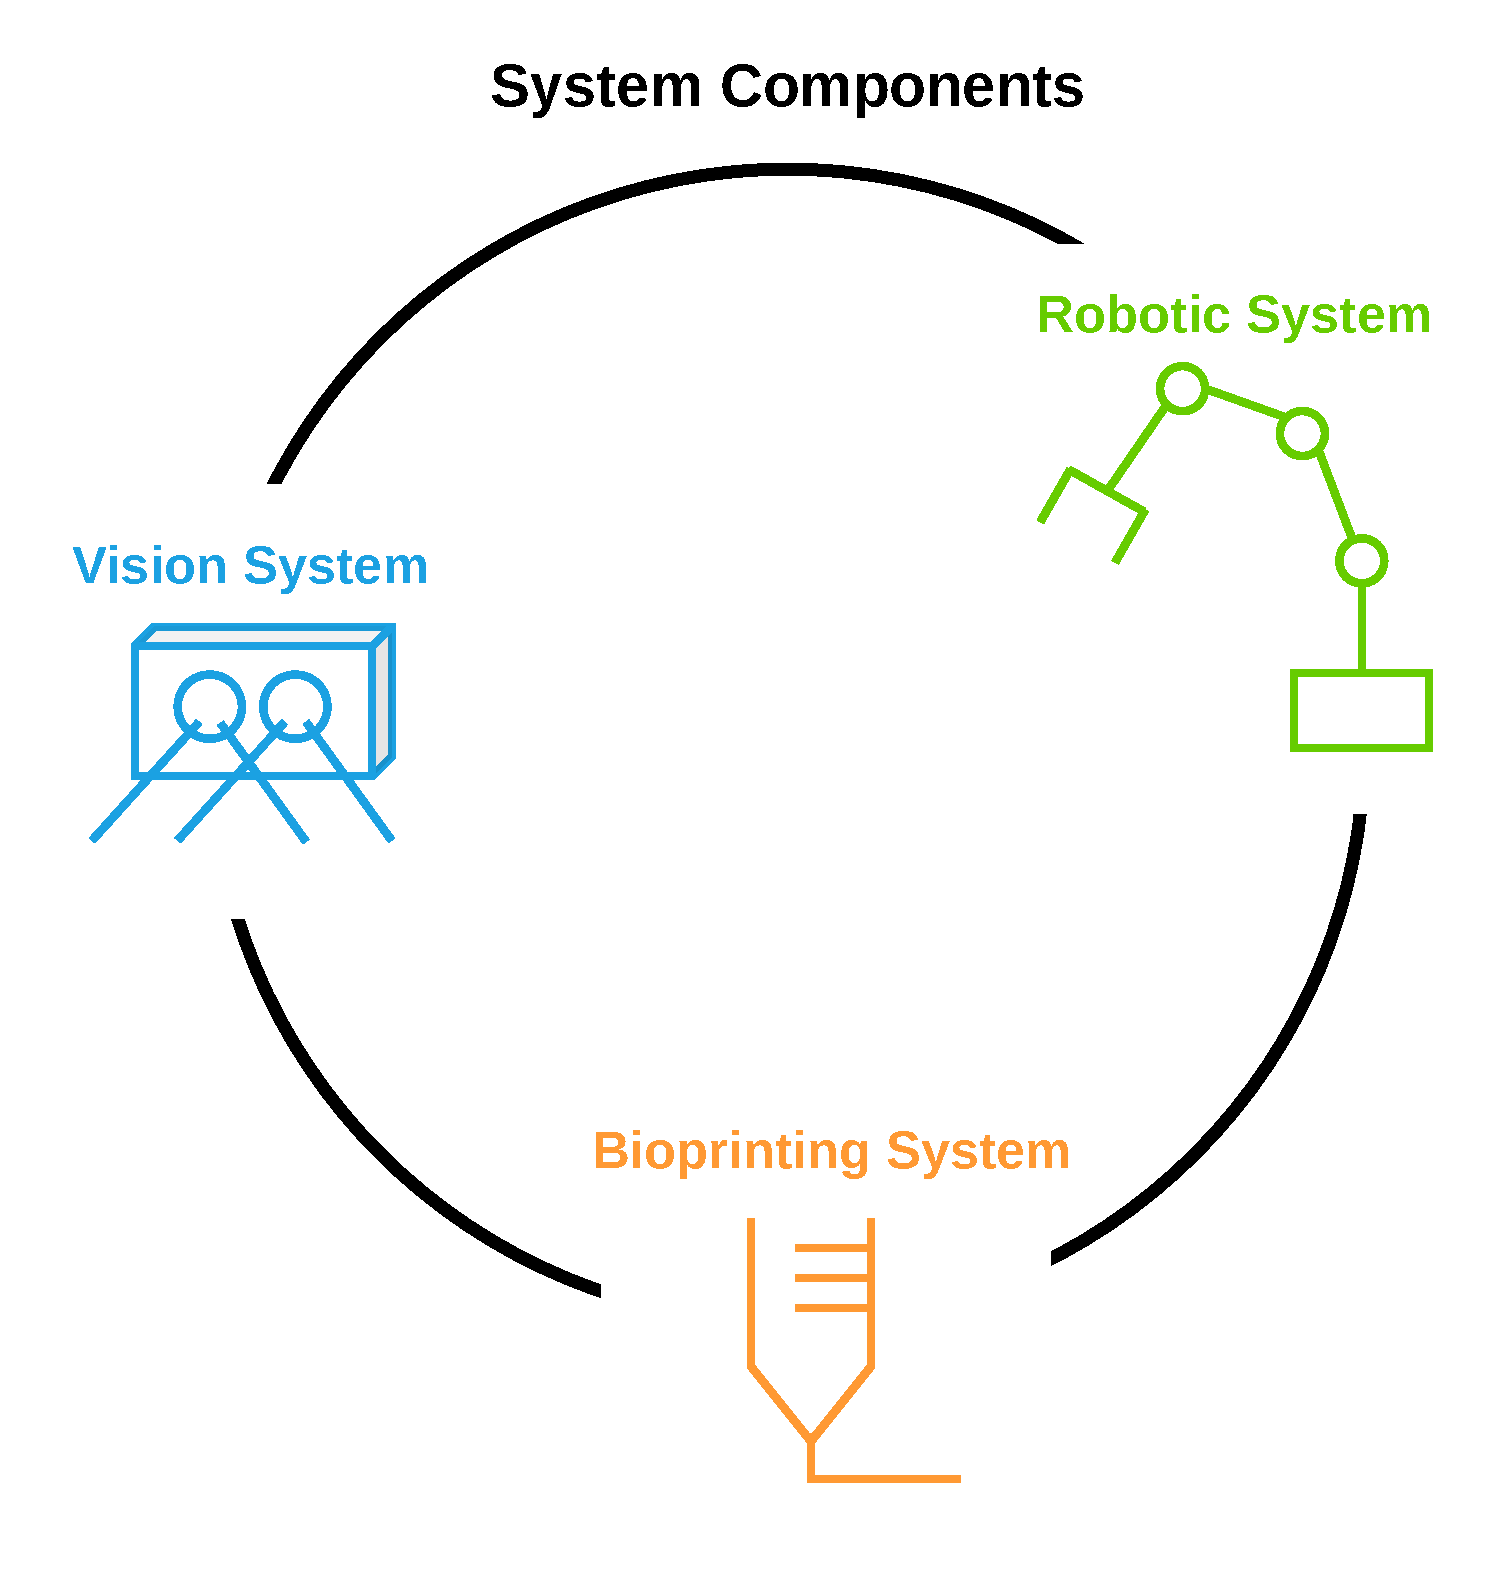
\includegraphics[width=.5\textwidth]{system_architecture_components_intro}
	\hspace{0.1in}
	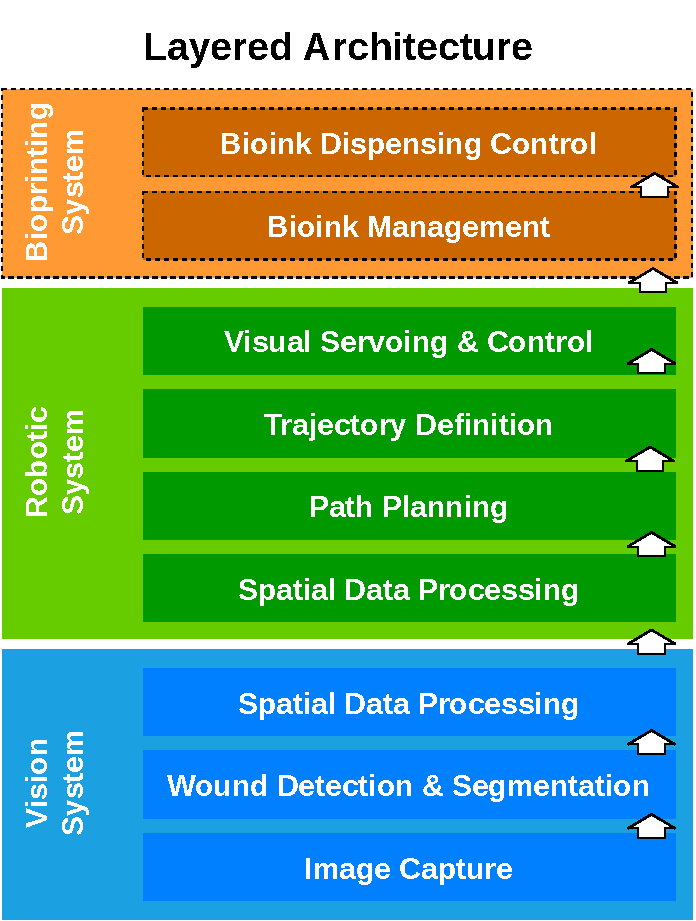
\includegraphics[width=.45\textwidth]{system_architecture_layers_intro}
	\caption{System architecture main components (left) and functional layers (right).}
	\label{fig:system_architecture_intro}
\end{figure}

The use of a robotic manipulator brings more \gls{dof}. This facilitates the process of bioprinting in non-planar surfaces. Using a camera makes possible to increase the autonomy of the bioprinting process. The combination of both systems facilitates the 3D bioprinting to be done in situ, as opposed to be inside the printer and then transferred to the final location.

A layered structure is used to describe the system's functional architecture. Composed by seven layers (Fig. \ref{fig:system_architecture_intro}), it aims to organise the system into independent modules that communicate between adjacent layers. Each layer provides a specific \gls{api} to the next layer.

On chapter \ref{cha:system_architecture}, the system architecture will be described in more detail.

% section proposed_system_architecture

% ======================
% = Document structure =
% ======================
\section{Document structure}
\label{sec:document_structure}

The document structure followed aims to guide the reader from the need of the proposed system, to its implementation, and ending on the results obtained and future needs. The thesis is organised into eight interdependent, but self-contained, chapters:

\begin{enumerate}
    \item \textbf{Introduction}, presents the biomedical application context of the proposed tool system, which is the reality of burn injury. It is followed by a summary of the current state of three different scientific fields that contribute for the development of the proposed tool. Afterwards, the goal of the thesis and a summary of the proposed system architecture are presented. It ends with the description of the thesis document's structure.
    
    \item \textbf{Theoretical Concepts}, introduces the fundamental concepts necessary for understanding the contents of this thesis. It focuses on concepts of robotic control and computer vision. 
    
    \item \textbf{Literature Review}, consists on an analysis of the current literature related with 3D bioprinting using robotic manipulators, with or without vision systems.
    
    \item \textbf{System Architecture}, is a full description of the proposed system architecture introduced on the first chapter. It starts with a description of the system requirements. Subsequently, the robotic system and the vision system are introduced. Finally, the system's interaction layers are described in detail.
    
    \item \textbf{Robotic System}, starts with a main overview of the robotic system. It describes the robot kinematic and dynamic characteristics. It ends with the integration of the robot with the \gls{ros} and Gazebo simulation environment.
    
    \item \textbf{Vision System}, describes the camera system used and the way it interfaces with the robot manipulator. It also describes the \gls{sdk} and the integration with \gls{ros} and Gazebo.
    
    \item \textbf{Control Architectures}, discusses several control architectures used for robot positioning and for visual servoing. Visual servoing is the use of visual input for control purposes.
    
    \item \textbf{System Validation}, is where all the test procedures are documented and results presented. It ends with a discussion of the results.
    
    \item \textbf{Conclusions}, presents the main conclusions of the thesis, and proposes future work.
\end{enumerate}

The document also has appendixes and annexes that complement the main body of text present on the previous chapters.

% section document_structure